\chapter{Wprowadzenie do dziedziny (Karina Wołoszyn)}
\label{chap:field}

Wzrost popularności gier w ostatnich latach szczególnie uwidocznił się podczas pandemii COVID-19, kiedy miliony ludzi zmieniły swój tryb życia, spędzając większość czasu w domach. Aby zaspokoić nudę w tak ograniczonych warunkach, wielu zwróciło się ku grom - największej spośród form rozrywki. Sytuacja ta przyczyniła się zarówno do powiększenia grupy konsumentów, jak i do wykształcenia nowych nawyków - wzmożonej aktywności w grach, utrzymującej się nawet po powrocie do normalnego stylu życia, bez ograniczeń wynikających z panujących wtedy restrykcji. Jednym z gatunków, które zyskały na popularności, były gry przeglądarkowe oraz gry geolokalizacyjne.

\section{Rynek gier przeglądarkowych}

Gry przeglądarkowe to rodzaj gier online, które nie wymagają użycia oddzielnych konsol - do ich uruchomienia wystarczy przeglądarka internetowa, dostępna zarówno na komputerach stacjonarnych, jak i na urządzeniach mobilnych. Charakteryzują się łatwym dostępem, niewielkimi wymaganiami sprzętowymi, brakiem potrzeby instalacji dodatkowego oprogramowania oraz niską ceną lub całkowitą darmowością. Rozgrywka w takich grach jest zazwyczaj podzielona na krótkie sesje, których celem jest przyciągnięcie i utrzymanie uwagi gracza. Popularność gier przeglądarkowych wynika również z możliwości gry wieloosobowej oraz wprowadzenia elementów rywalizacji, takich jak rankingi.

Gry przeglądarkowe istnieją niemal od początku Internetu, czyli od lat 90. XX wieku.Szczególną uwagę należy jednak poświęcić latom dwutysięcznym, kiedy firma Adobe Systems przejęła Macromedię i rozwijała produkt Adobe Flash. Flash zrewolucjonizował rynek gier, umożliwiając niezależnym twórcom i małym studiom produkcję niewielkich gier działających na większości komputerów i przeglądarek. Do najpopularniejszych gatunków gier przeglądarkowych należą m.in. gry MMO (ang. \textit{massively multiplayer online}), w których gracze z całego świata łączą się, aby wspólnie eksplorować i oddawać się immersji w świecie stworzonym przez twórców.

Przykładem gry MMO jest Travian wydany w 2004 roku, który jest jedną z najpopularniejszych gier przeglądarkowych. W Travian gracze wcielają się w rolę przywódców wiosek, rozwijając swoje imperia poprzez zbieranie surowców, budowanie struktur oraz prowadzenie wojen z innymi graczami. Gra oferuje różnorodne strategie, a interakcje między graczami są kluczowym elementem rozgrywki, co sprawia, że Travian cieszy się dużą popularnością od wielu lat.

\begin{figure}[H]
    \centering
    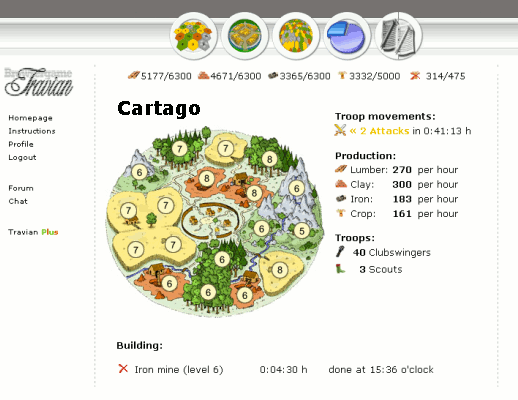
\includegraphics[width=0.5\textwidth]{images/travian.png}
    \caption{Gra Travian wydana w 2004 roku.\protect\footnotemark[1]}
    \label{fig:travian}
\end{figure}

Gry takie jak Club Penguin \ref{fig:club_penguin}, które zadebiutowały w 2005 roku, przyciągnęły rzesze fanów, budując społeczność i poczucie wspólnoty. W tej grze gracze mogli tworzyć własne postacie, eksplorować wirtualny świat, uczestniczyć w różnych mini-grach oraz wchodzić w interakcje z innymi graczami. Gra stała się symbolem gier społecznościowych, a jej zamknięcie w 2017 roku pozostawiło wielu graczy z nostalgią za wspólnie spędzonym czasem w tym wirtualnym świecie. Co podkreśla fakt jak ważne jest dla graczy, szczególnie przeglądarkowych, posiadać możliwość integrowania się w świecie wirtualnym.

\begin{figure}[H]
    \centering
    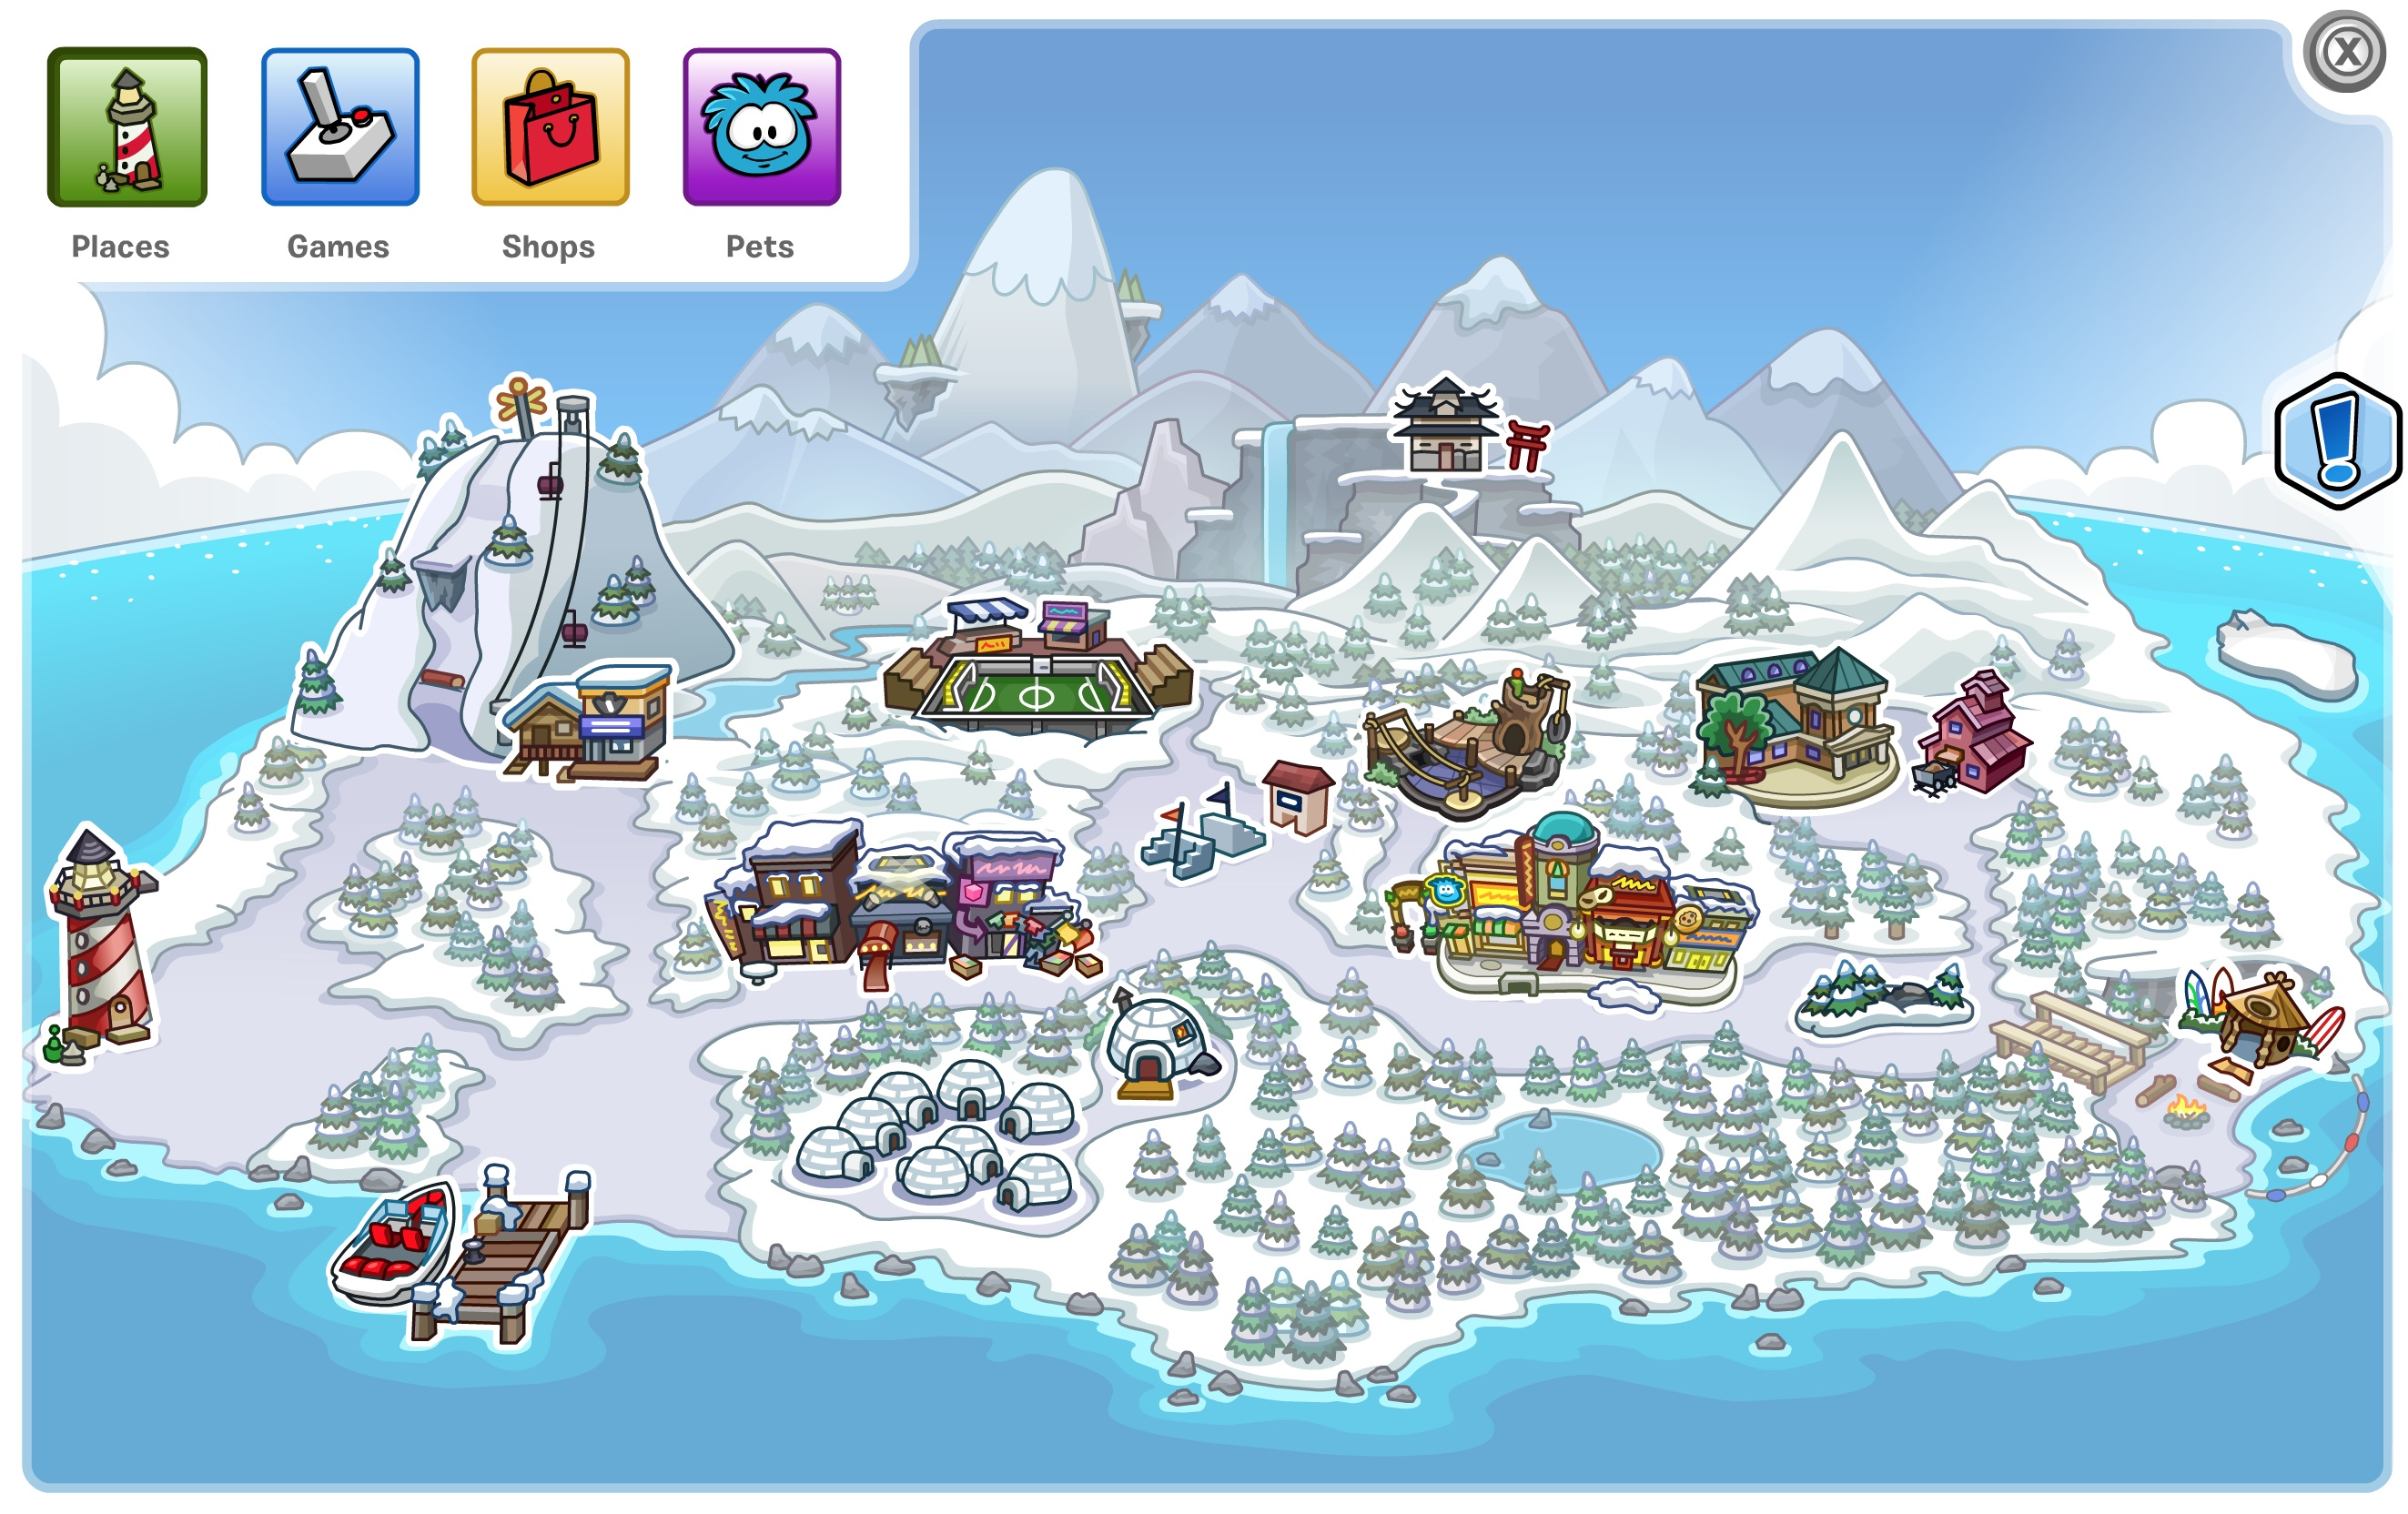
\includegraphics[width=0.5\textwidth]{images/club_penguin.jpeg}
    \caption{Gra Club Penguin wydana w 2005 roku.\protect\footnotemark[2]}
    \label{fig:club_penguin}
\end{figure}

Gry typu .io to produkcje o prostej mechanice, w których gracze rywalizują online na ograniczonej arenie. Charakteryzują się minimalistyczną grafiką, prostymi zasadami i krótkimi sesjami rozgrywki. Popularność tego gatunku zapoczątkowała gra Agar.io \ref{fig:agario}, stworzona w 2015 roku przez brazylijskiego dewelopera. Gracz steruje w niej jedną (lub wieloma) jednokolorowymi komórkami, których celem jest zdobycie jak największej masy. Aby to osiągnąć, należy unikać większych komórek i zjadać mniejsze.

\begin{figure}[H]
    \centering
    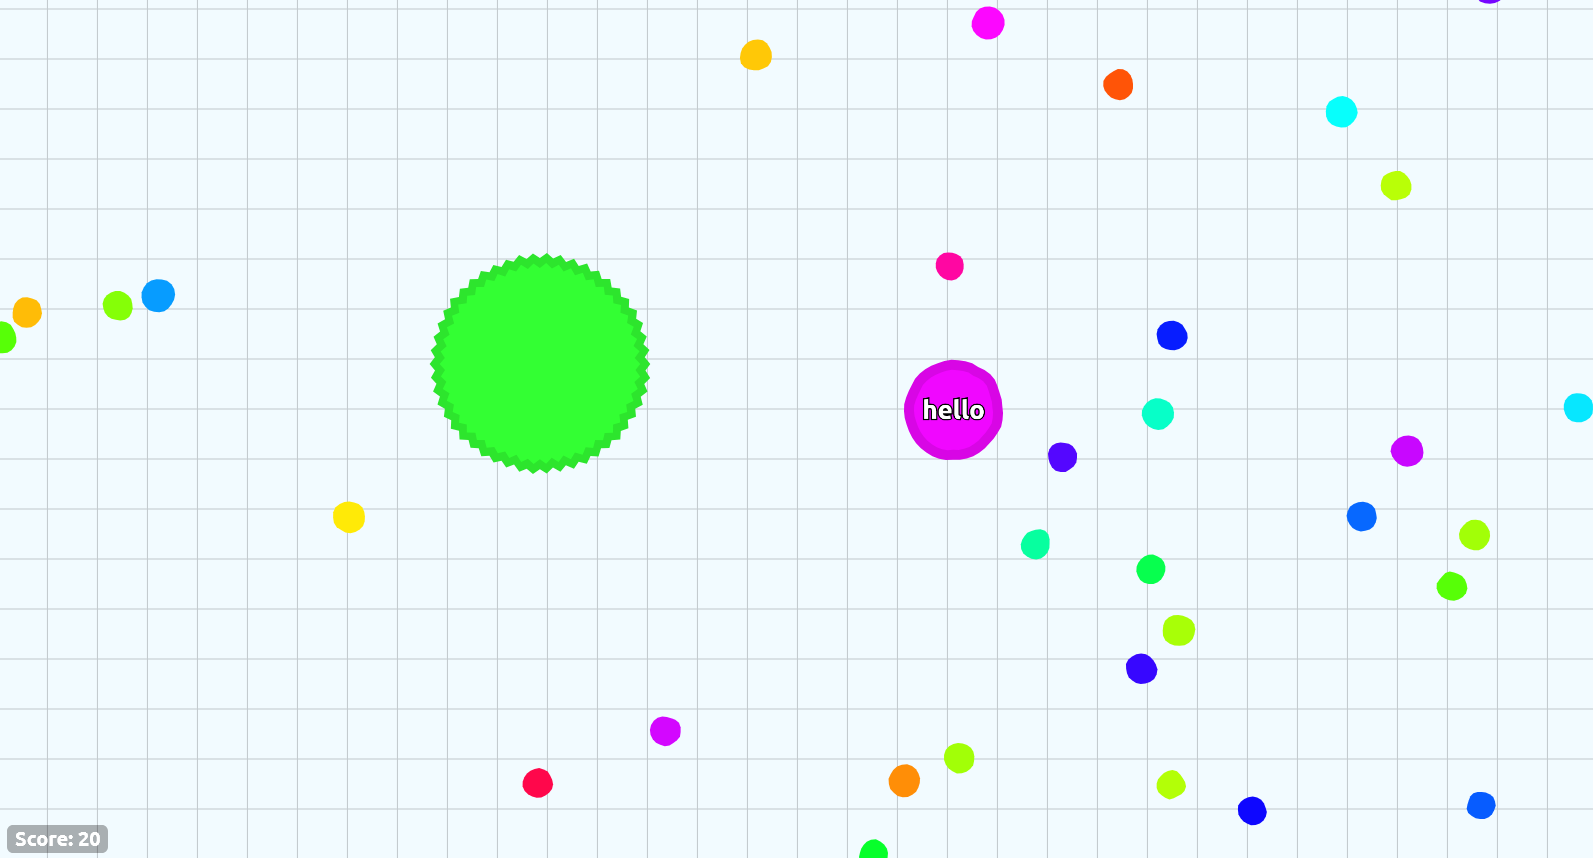
\includegraphics[width=0.5\textwidth]{images/agario.png}
    \caption{Gra Agar.io wydana w 2015 roku.\protect\footnotemark[3]}
    \label{fig:agario}
\end{figure}

Na popularności gry Agar.io zyskały również inne produkcje, oparte na podobnej mechanice. W Slither.io \ref{fig:slitherio} gracz steruje wężem, który zwiększa swoją masę poprzez zjadanie komórek. Oprócz tego może pokonać większych rywali, blokując im drogę i eliminując ich, a następnie przejmując ich komórki. Wąż ma również możliwość tymczasowego przyspieszenia - ruch ten pozwala szybciej manewrować po arenie i atakować innych graczy, jednak każdorazowe użycie przyspieszenia powoduje utratę części masy węża, co wymaga strategicznego zarządzania zasobami, aby nie osłabić własnej pozycji.

\begin{figure}[H]
    \centering
    
\includegraphics[width=0.5\textwidth]{images/slitherio.png}
    \caption{Gra Slither.io wydana w 2016 roku.\protect\footnotemark[4]}
    \label{fig:slitherio}
\end{figure}

Wraz z rozwojem przeglądarek gry, które na nich działały, zyskiwały na szybkości przetwarzania animacji i innych elementów graficznych, a także na wydajności i złożoności rozgrywki. Z biegiem lat zmieniały się również sposoby zarządzania pamięcią i obsługi technologii - obok gier działających w Adobe Flash pojawiły się produkcje oparte na HTML5 (ang. \textit{HyperText Markup Language}), JavaScript i WebGL, a następnie rozwinięto koncepcję PWA (\textit{Progressive Web App}), czyli progresywnych aplikacji umożliwiających działanie zarówno jako natywne aplikacje mobilne, jak i desktopowe.

\newpage

\section{Rynek gier geolokalizacyjnych}

Gry geolokalizacyjne wykorzystują dane lokalizacyjne gracza oraz informacje satelitarne, łącząc świat rzeczywisty z cyfrowym. Mechanika tych gier opiera się na precyzyjnym wykorzystaniu GPS (ang. \textit{Global Positioning System}), eksploracji otoczenia oraz elementach rywalizacji. Gry te wyróżniają się dokładnymi danymi lokalizacyjnymi i przedstawianiem ich w formie interaktywnej mapy, co pozwala na nowe doświadczenia w rozrywce i interakcji społecznej.

Jednym z najbardziej rozpoznawalnych tytułów jest GeoGuessr \ref{fig:geoguessr}, który znacząco zyskał na popularności dopiero siedem lat po premierze, czyli podczas pandemii COVID-19 w 2020 roku. Gra pozwala na eksplorowanie świata bez wychodzenia z domu - zadaniem gracza jest poprawne odgadnięcie lokalizacji przedstawionego miejsca w ograniczonym czasie, zaznaczając swoją odpowiedź na interaktywnej mapie. Popularność GeoGuessr w tym okresie pokazuje, jak pandemia zmieniła nawyki konsumenckie i zwiększyła zainteresowanie grami wymagającymi zarówno spostrzegawczości, jak i wiedzy geograficznej.

\begin{figure}[H]
    \centering
    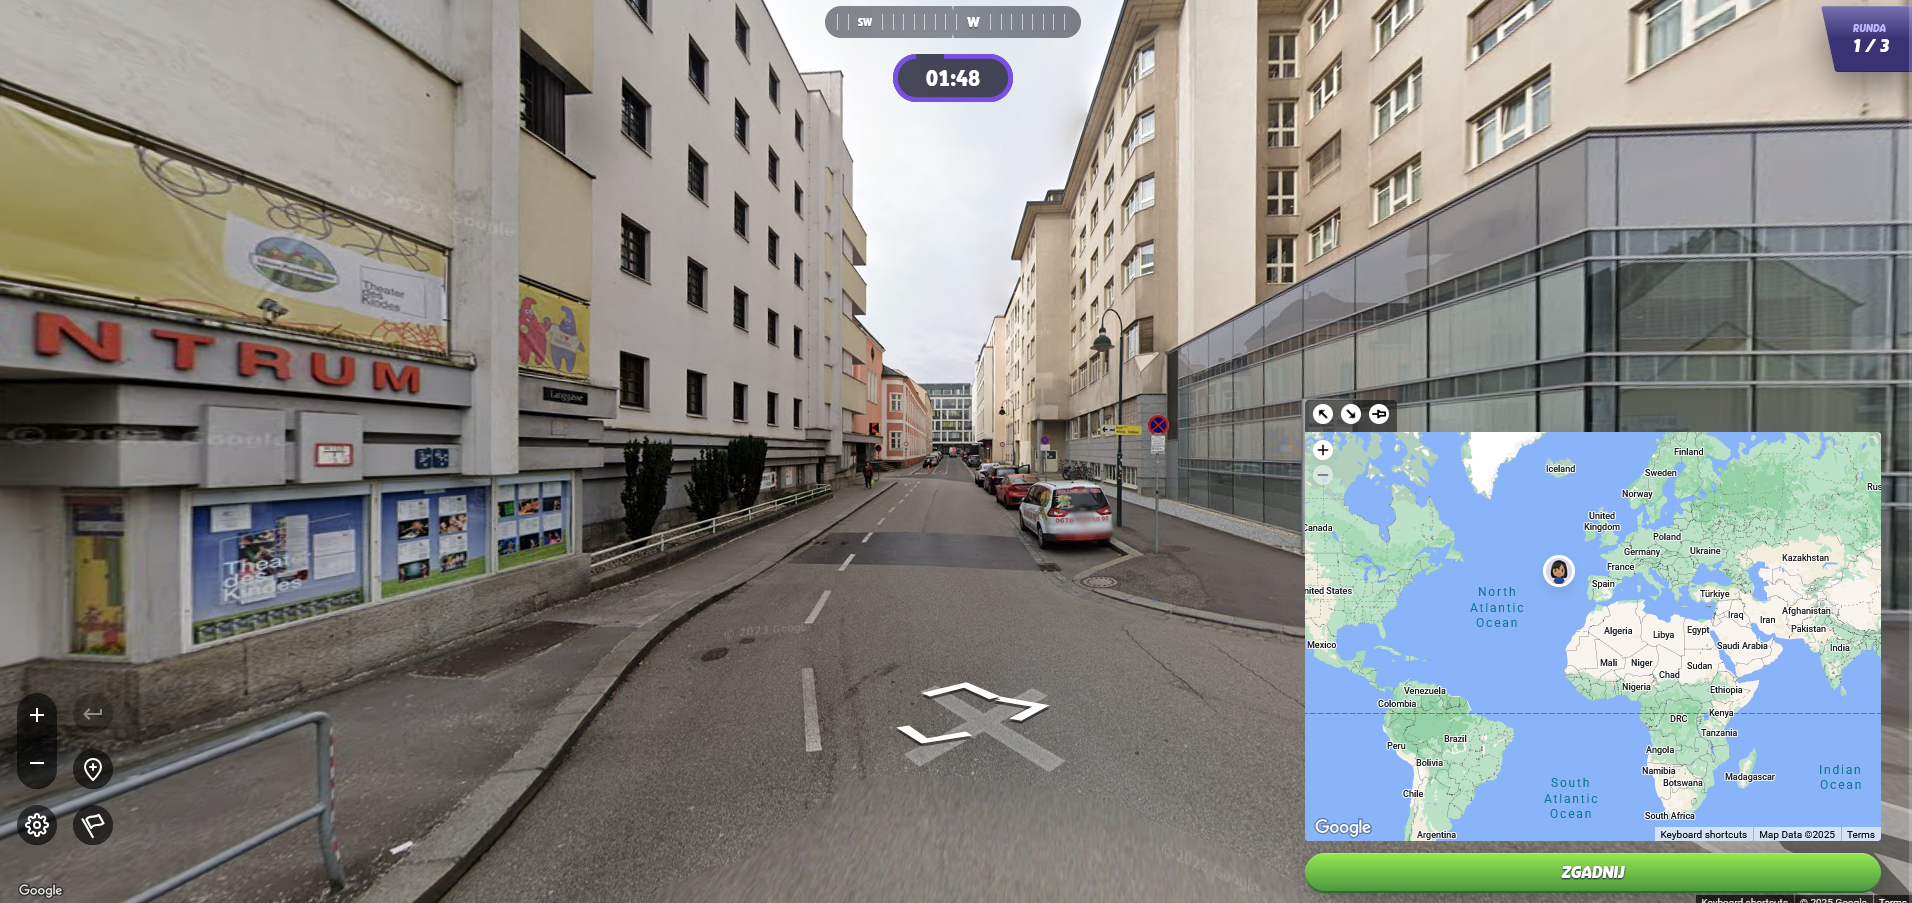
\includegraphics[width=0.5\textwidth]{images/geogussr.png}
    \caption{Gra Geoguessr wydana w 2020 roku.\protect\footnotemark[5]}
    \label{fig:geoguessr}
\end{figure}

Innym przykładem jest mobilna gra Pokémon GO \ref{fig:pokemongo}, stworzona przez firmę Niantic, Inc. i wydana w 2016 roku. Gra opiera się na technologii AR (ang. \textit{Augmented Reality}) i pozwala graczom eksplorować swoje otoczenie w poszukiwaniu Pokémonów, łączyć wirtualny świat z rzeczywistym oraz wchodzić w interakcje z innymi graczami przy specjalnych punktach, takich jak PokéStopy czy Gymy. Pokémon GO jest częścią szeroko znanej franczyzy Pokémon, co znacząco przyczyniło się do popularyzacji gry i zwiększenia jej zasięgu, przyciągając zarówno fanów marki, jak i nowych graczy zainteresowanych nowatorską mechaniką AR.

\begin{figure}[H]
    \centering
    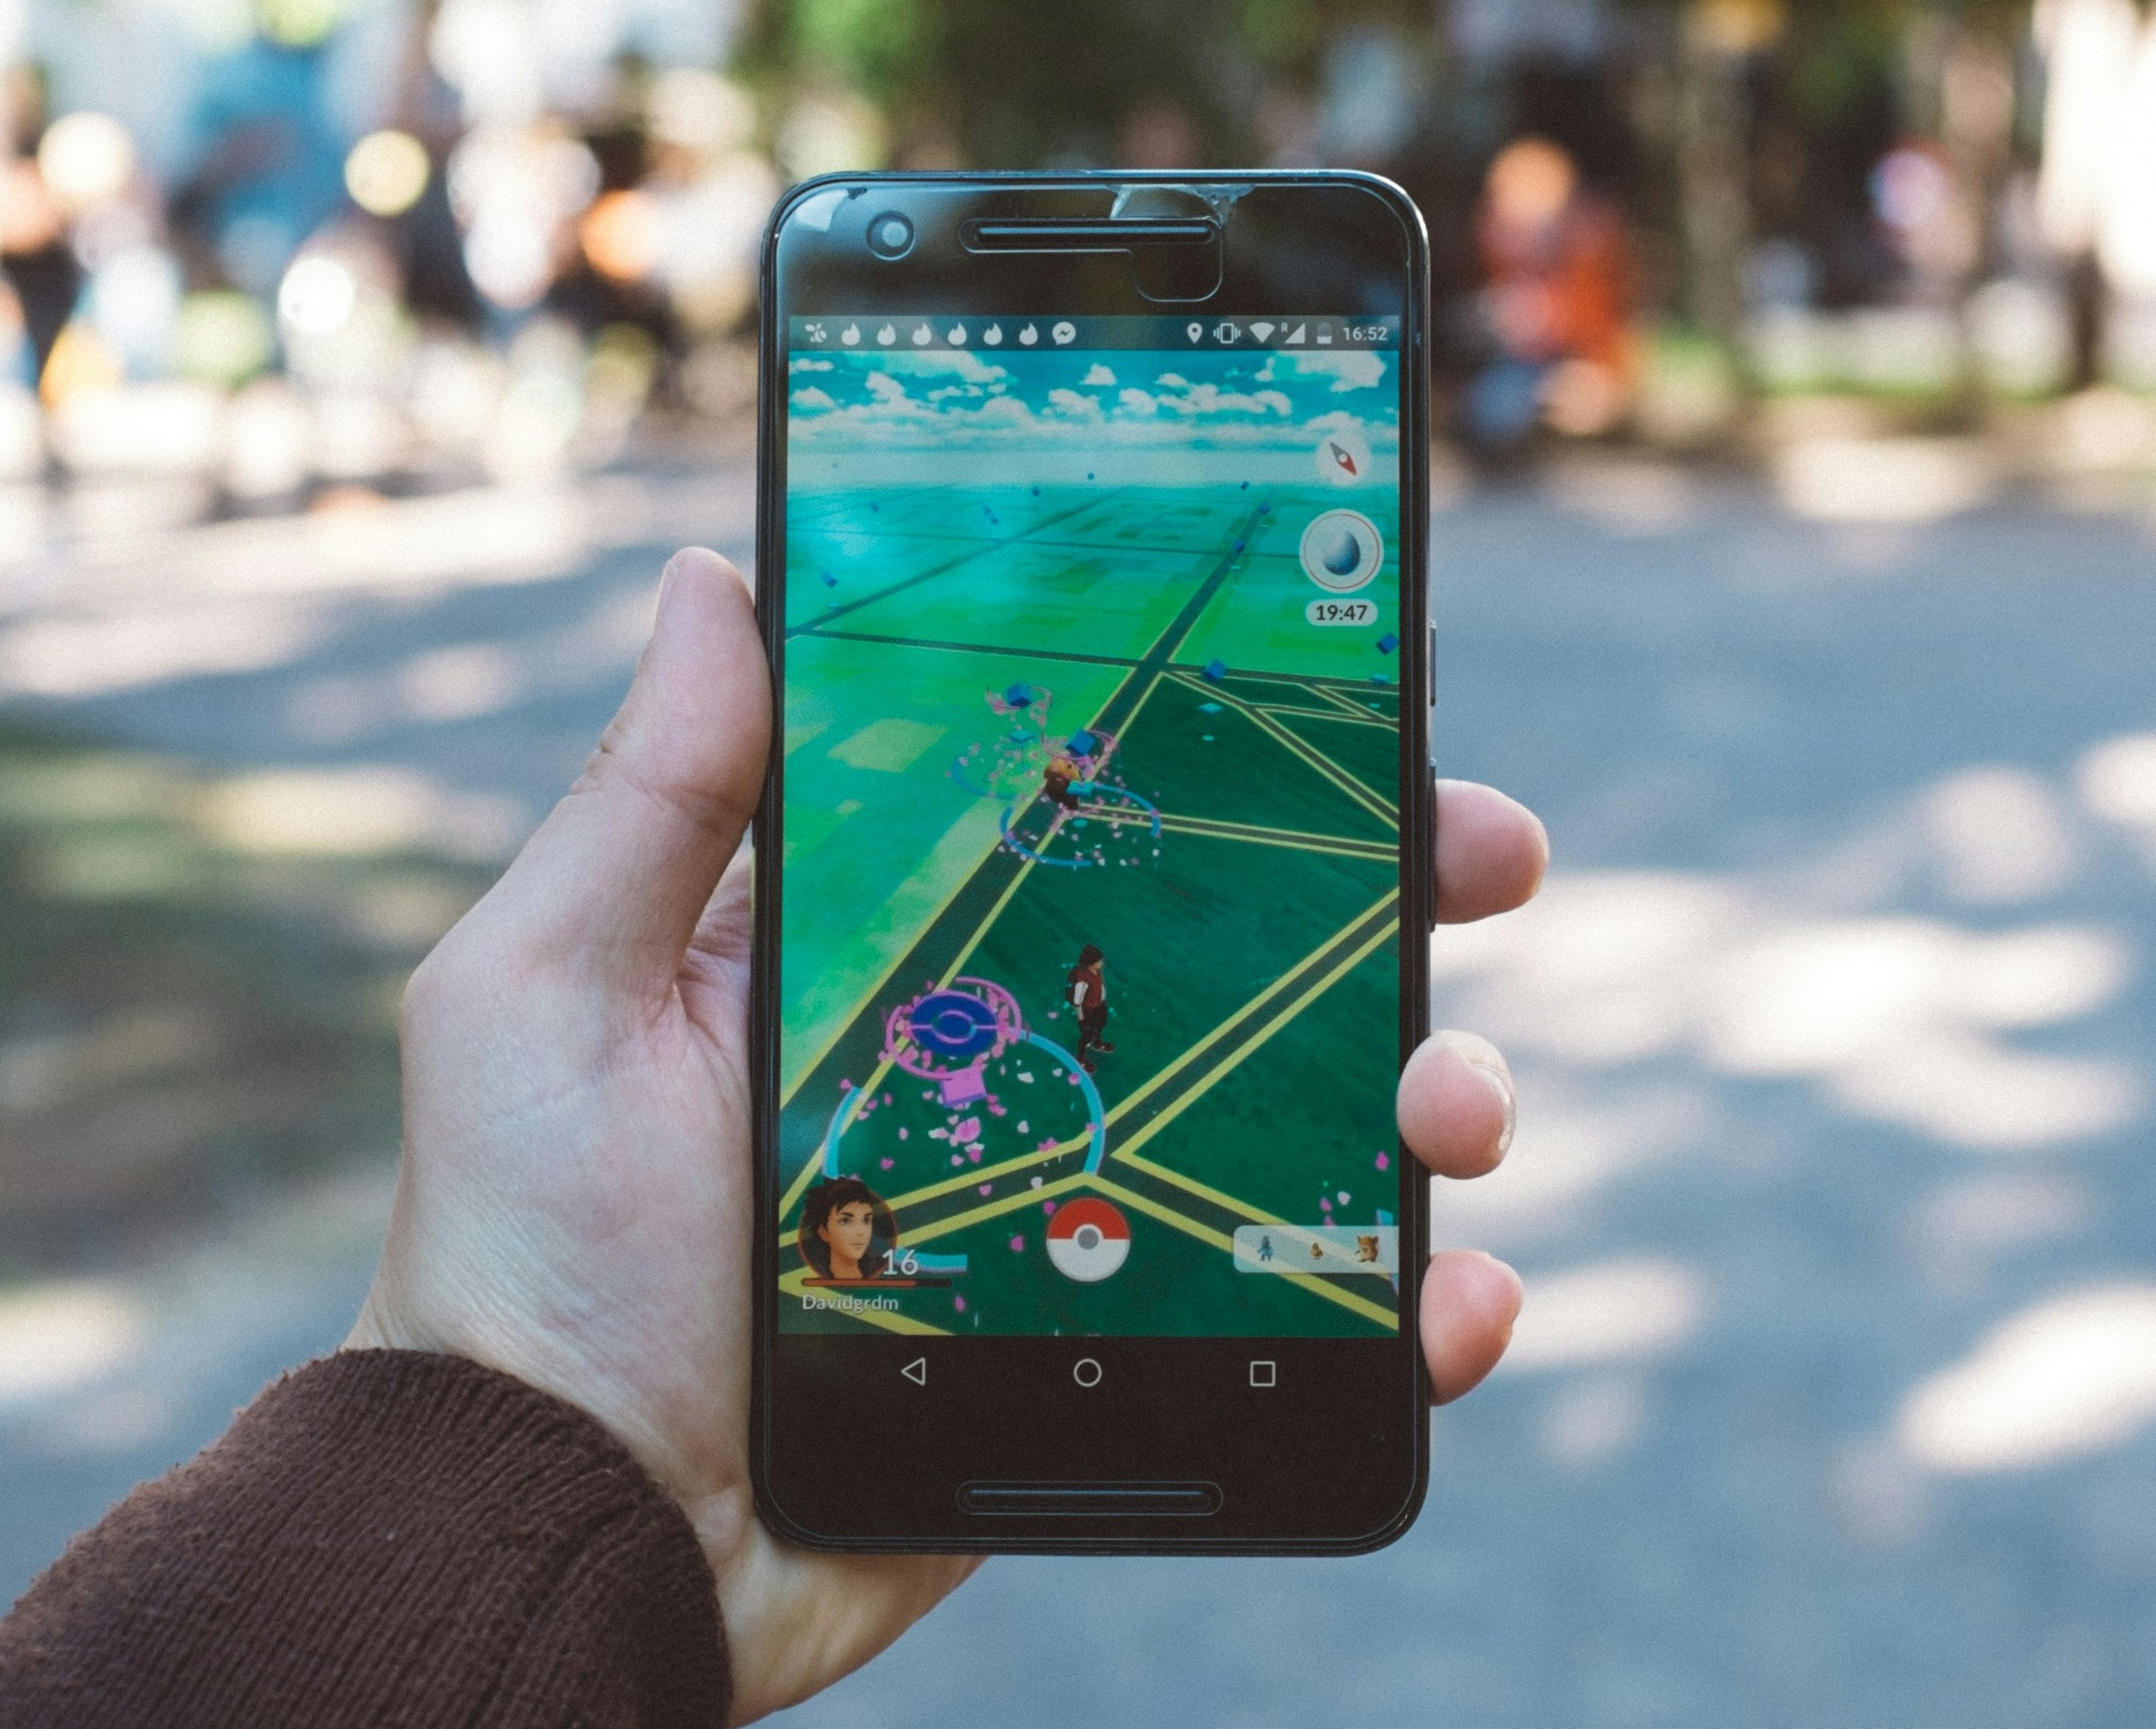
\includegraphics[width=0.5\textwidth]{images/pokemongo.jpg}
    \caption{Gra PokemonGO wydana w 2016 roku.\protect\footnotemark[6]}
    \label{fig:pokemongo}
\end{figure}

\newpage

Z kolei Back of Your Hand \ref{fig:backofyourhand} skupia się na znajomości własnej okolicy i charakterystycznych obiektów. Gracz otrzymuje jedynie nazwę ulicy lub konkretnego miejsca, a następnie w określonym obszarze (np. w promieniu 1500 metrów) musi odnaleźć je na mapie. Im bliżej poprawnej lokalizacji gracz umieści swój „strzał”, tym więcej punktów zdobywa. Po zakończeniu rundy wyświetlane jest podsumowanie, w którym wszystkie miejsca i trafienia gracza prezentowane są na jednej interaktywnej mapie, umożliwiając łatwe przeanalizowanie wyników i strategii.

\begin{figure}[h]
    \centering
    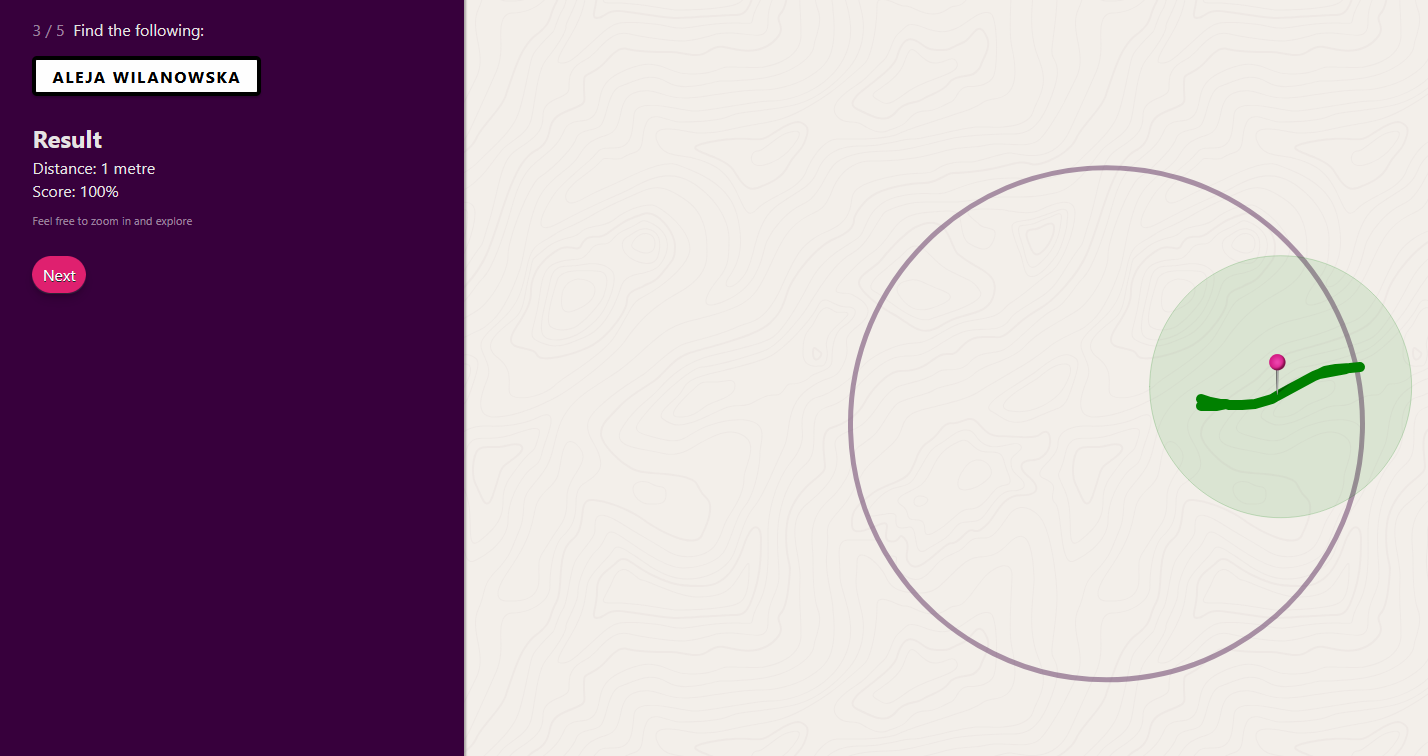
\includegraphics[width=0.5\textwidth]{images/backofyourhand.png}
    \caption{Gra Back of Your Hand wydana w 2020 roku.\protect\footnotemark[7]}
    \label{fig:backofyourhand}
\end{figure}

\section{Rodzaje gier konkurencyjnych}

Gry konkurencyjne to tytuły oparte na rywalizacji między graczami, w których często pojawiają się takie elementy jak rankingi, historia rozgrywek, tryby turniejowe czy codzienne wyzwania. Do tego typu gier można zaliczyć nie tylko wcześniej wspomnianego GeoGuessr, ale również produkcje takie jak Geotastic \ref{fig:geotastic} czy Tetris 99 \ref{fig:tetris}.

Geotastic to gra bardzo zbliżona pod względem mechaniki do GeoGuessr. To, co przyciągnęło miliony graczy, to fakt, że jest darmową alternatywą, oferującą innowacyjne tryby rozgrywki oraz opartą na finansowaniu społecznościowym. Zaangażowana społeczność graczy aktywnie uczestniczy w rozwoju gry, dbając o jej aktualizację i utrzymanie, co dodatkowo wzmacnia jej atrakcyjność i trwałość w dłuższym okresie.

\begin{figure}[H]
    \centering
    
\includegraphics[width=0.5\textwidth]{images/geotastic.png}
    \caption{Gra Geotastic wydana w 2020 roku.\protect\footnotemark[8]}
    \label{fig:geotastic}
\end{figure}

Bazując na znanej serii Tetris, twórcy Tetris 99 rozszerzyli koncepcję klasycznej gry logicznej o formułę battle royale. W tym trybie jednocześnie rywalizuje ze sobą 99 graczy, układając spadające klocki na własnych planszach. Gracze eliminują kolejne linie poprzez ich całkowite wypełnienie, a usunięte bloki są następnie wysyłane jako tzw. garbage lines do wybranych przeciwników. Zwycięzcą zostaje osoba, która najdłużej utrzyma się w grze i jako ostatnia będzie w stanie wykonać legalny ruch. \\Tytuł odwołujący się do klasycznej, jednoosobowej rozgrywki szybko zyskał popularność. Mimo że został wydany wyłącznie na konsolę Nintendo Switch, niemal natychmiast zdobył uznanie graczy i krytyków. Już w pierwszych miesiącach od premiery otrzymał nagrodę \textit{Best Multiplayer Game of 2019} przyznaną przez serwis Shacknews~\cite{shacknews-tetris}, a do kwietnia 2019 roku został uruchomiony na ponad 2,8 miliona kont. Sukces Tetris 99 udowadnia, że nawet klasyczny koncept, odpowiednio odświeżony, wzbogacony o nowoczesną formułę rywalizacji oraz dopracowaną mechanikę, może ponownie stać się atrakcyjny i odnieść znaczący sukces rynkowy.

\begin{figure}[htbp]
    \centering
    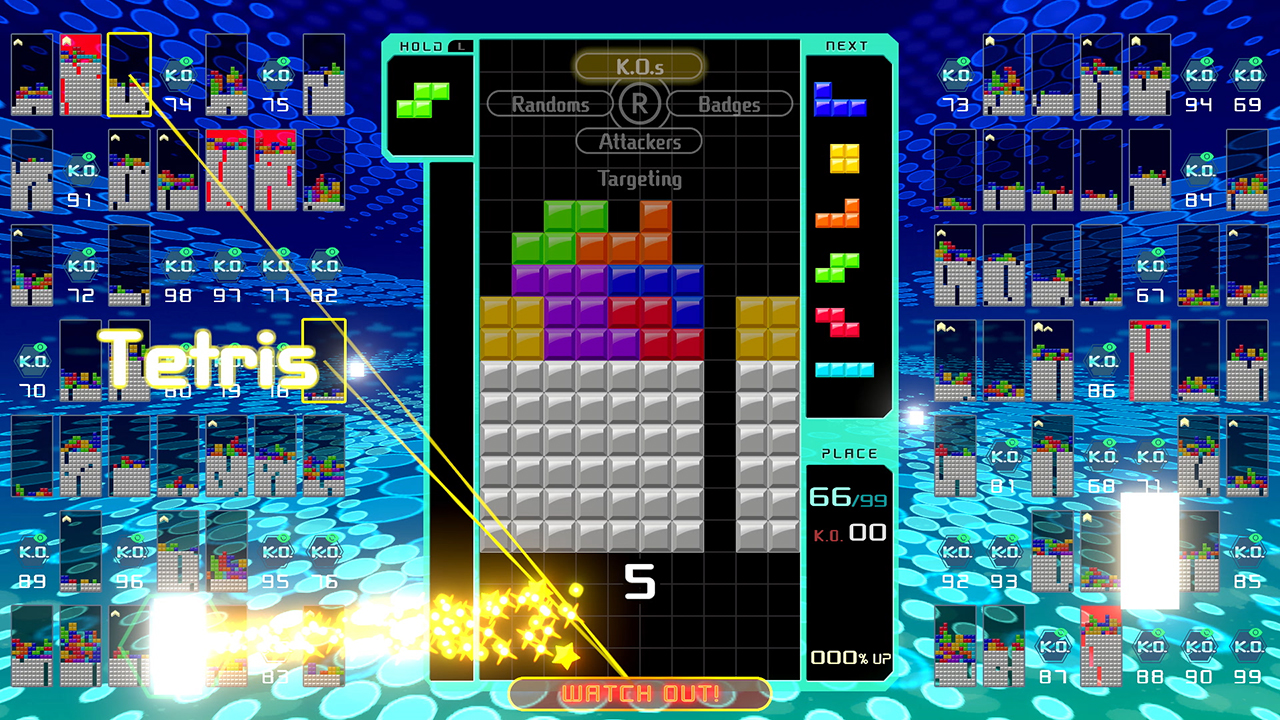
\includegraphics[width=0.5\textwidth]{images/tetris.jpg}
    \caption{Gra Tetris 99 wydana w 2019 roku.\protect\footnotemark[9]}
    \label{fig:tetris}
\end{figure}

\footnotetext[1]{Źródło: \url{https://www.uvlist.net/game-167566-Travian}}
\footnotetext[2]{Źródło: \url{https://fontsinuse.com/uses/7135/club-penguin-2005-14}}
\footnotetext[3]{Zdjęcie wykonane samodzielnie. Gra dostępna pod adresem: \url{https://www.agar.io/}}
\footnotetext[4]{Zdjęcie wykonane samodzielnie. Gra dostępna pod adresem: \url{https://www.slither.io/}}
\footnotetext[5]{Zdjęcie wykonane samodzielnie. Gra dostępna pod adresem: \url{https://www.geoguessr.com/}}
\footnotetext[6]{Źródło: \url{https://unsplash.com/photos/person-playing-pokemon-go-during-daytime-Am1io6KusFM}}
\footnotetext[7]{Zdjęcie wykonane samodzielnie. Gra dostępna pod adresem: \url{https://backofyourhand.com}}
\footnotetext[8]{Zdjęcie wykonane samodzielnie. Gra dostępna pod adresem: \url{https://geotastic.net/home}}
\footnotetext[9]{Źródło: \url{https://cdn.arstechnica.net/wp-content/uploads/2019/02/7kimTJTFJQf0Ohb2_jjt0oKVJ22VSgga.jpg}}
